\section{Wide column}
L'idea è che accanto a la chiave non ho un valore/blob ma ho una riga con degli attributi mono-valore. Si ha quindi una via di mezzo tra il modello \textit{key-value} e il modello documentale. \\ 
Ci sono diversi modelli di tipo colonnare \textbf{column}: bigTable, Hbase, Cassandra e altri.
\subsection{bigTable}
L'idea dietro \textbf{BigTable} è quella di una mappa multidimensionale ordinata, persistente e sparsa, ovvero si ha una mappa indicizzata tramite tre informazioni: row key, column key, timestamp. I timestamp servono per andare a vedere il momento in cui è stata attuata una modifica. All'interno si hanno poi varie \textbf{column family} con i vari dati, memorizzati come \textit{string}.\\ BigTable è molto usato in ambito web grazie alla sua capacità di memorizzare anche contenuti HTML\\
Grazie ai timestamp si garantisce un controllo di concorrenza basato sul multiversioning. Possiamo dire che i sistemi che implementano \textit{wide column} con timestamp supportano transazioni ACID tramite protocollo \textbf{MultiVersion Concurrency Control (\textit{MCC o MVCC})}.\\
Un insieme di righe viene definito \textbf{tablet}. Abbiamo visto che ogni riga può avere diversi \textbf{column family} e si ha che ciascun column family può avere diversi \textbf{qualifier} e per ogni qualifier più valori diversi in base al timestamp. La libertà dello schema deriva che ogni column family può avere un numero diverso di qualifier. Si ha quindi l'approccio \textit{key-value} per l'accesso tramite chiave e si ha un sistema di indicizzazione per migliorare le prestazioni. Ogni column family ha un nome, una \textit{string}, è può contenere altre colonne, che a loro volta appartengono ad una column family, specificata tramite \texttt{familyName:columnName}. Il timestamp (anche se può essere usato altro) garantisce un \textbf{version number} univoco.
\subsection{Hbase}
La versione distribuita di BigTable venne rinominata \textbf{Hbase} (dove $H$ sta per \textbf{Hadoop}).\\ In questo caso i dati sono divisi in tables e ogni table è composta di colonne che sono a loro volta raggruppate in column family (che possono avere un numero variabile di colonne, che erano i qualifier in BigTable).Supporta quindi il multiversioning.\\
Un'istanza di Hbase è formata da varie righe, identificate tramite una chiave, a cui sono associate per ciascuna riga, varie column family, una per ogni tipo di dato. \\
La column family viene rappresentata tramite un insieme di coppie attributo-valore e i valori possono avere timestamp diversi, specificati tramite \texttt{@timestamp} (\texttt{@ts=value}).\\ Si possono avere le stesse column family, dal punto di vista del nome, in più righe ma queste possono avere un insieme diverso di valori, garantendo che la table è \textbf{sparse}, rivelandosi utile per il mapping uno a tanti. I dati sono tutti \textit{bytes}\\
\begin{figure}[H]
    \centering
    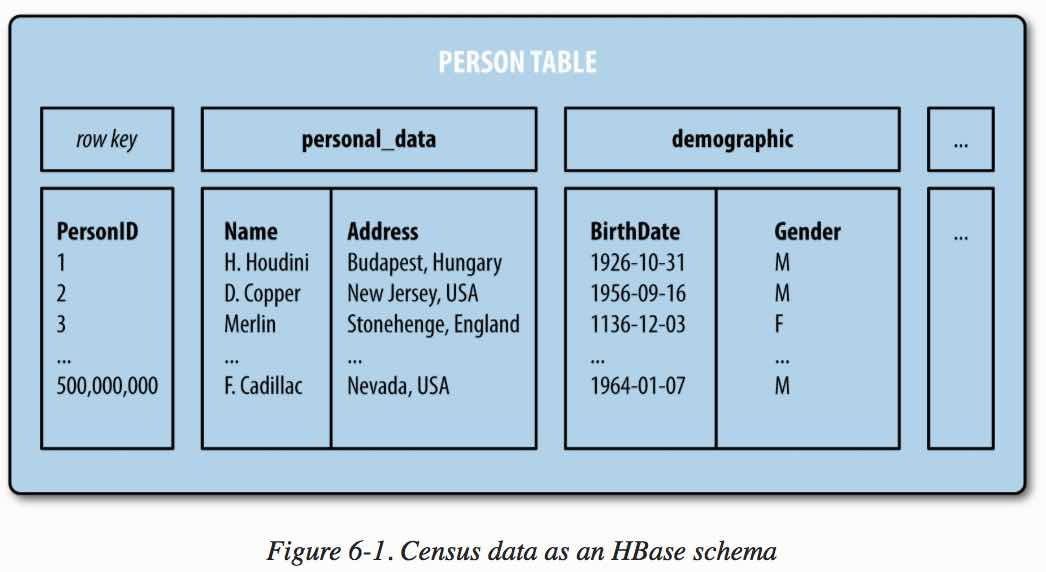
\includegraphics[scale = 0.26]{Immagini/hbasetable.jpg}
\end{figure}
Il modello colonnare non presta attenzione ai \textit{join}, che in questo caso implicherebbero scorrere l'intera tabella, ma si concentra sul \textbf{denormalizzare} ovvero a replicare le informazioni se devo fare dei join tra i vari elementi.\\
Quindi lo schema è formato dalle tables e dalle column family, \textbf{le colonne non fanno parte dello schema}.\\ 
Hbase implementa le \textbf{dynamic Columns} in quanto ogni riga ha differenti colonne.\\ Il versioning è essenziale per garantire lo storico delle informazioni. SU Hbase ho alcune operazioni fondamentali come aggiungere valori e ricercare per valore esatto (e non in modo range-based).\\

Vediamo quindi come si distribuisce un cluster Hbase. Si hanno tre componenti principali (ricordando che si basa su Hadoop), avendo un'architettura master/slave: 
\begin{enumerate}
  \item un master, detto \textbf{HbaseMaster}
  \item tanti region server, detti \textbf{HRegionServer}, che sono i vari slave
  \item il client, detto \textbf{Hbase client}, che dialoga con il singolo master 
\end{enumerate}
Nel dettaglio una \textit{region} è un sottoinsieme di righe della tabella, che vengono partizionate orizzontalmente tramite regole standard di frammentazione (partizionamento che viene fatto in automatico). Quindi un \textit{HRegionServer} gestisce un insieme di righe di una o più tabelle e la sincronizzazione avviene tramite file di log. Il master coordina gli slave, assegna le region, riconosce fallimenti degli slave. \\

Guardando l'intero diagramma il client fa la richiesta al master il quale cerca la posizione del dato e sviluppa l'operazione all'interno della singola region. Nel momento in cui il region server scrive i dati, attraverso il sistema distribuito chiamato \textbf{Hadoop Distributed File System (\textit{HDFS})}, viene fatta la replica e avviene il trasferimento delle informazioni dei file di log e quindi la sincronizzazione dei dati.\\
Potrei avere più master coordinati tra loro. Il coordinamento tra i master e i region server avviene tramite il meccanismo di \textbf{ZooKeeper}, ovvero un orchestratore software. HDFS permette di avere la memorizzazione orizzontale dei dati e tramite il \textbf{write ahead log (\textit{WAL})} prima scrivo sul log e poi sul disco, garantendo la ricostruibilità dei dati in caso di guasto e garantendo che prima o poi i dati saranno allineati. ZooKeeper quindi coordina master e region server per lettura/scrittura mentre HDFS consente l'allineamento dato che poi i dati vengono memorizzati su un file system distribuito.\\ 
Hbase ha un linguaggio di query poco ricco, potendo fare solo una \textit{select} di dati con un certo valore. Si può comunque fare la ricerca sia sulle righe che su alcuni attributi (definiti precedente come chiave). Il sistema di ricerca è estremamente performante.
\subsection{Cassandra}
Come abbiamo detto \textbf{Cassandra} lo studiamo come modello \textit{wide column} anche se loro stessi si definiscono anche \textit{key-value}, essendo sostanzialmente tale ma usando concetti dei modelli \textit{wide column}.\\ Cassandra è l'evoluzione open source del db NoSQL utilizzato da Facebook e risulta interessante perché implementa un sistema di distribuzione completamente diverso da quello master/slave di Hbase.\\ In cassandra esiste il concetto \textbf{column family}, definito all'interno di un \textbf{key space}, come insieme di coppie key-value e quindi una column family altro non è che una tabella con le coppie key-value come righe. Ogni riga ha poi assocciato un $Row Id$ che la identifica.(scritto su slide)\\ Il concetto di column family quindi varia rispetto a quello di Hbase. Una riga è una collezione di colonne con un nome, il $Row id$. La chiave corrisponde al nome della colonna e ogni riga contiene almeno una colonna.\\

Si possono aggiungere attributi a piacere e modificarli (mentre in Hbase si creavano/modificavano le column family). Se i valori corrispondenti a tutte le column name sono uguali a \textbf{-} si specifica che essi non sono usati. Posso anche specificare di avere un singolo valore non in uso sempre con \textbf{-}. Il linguaggio di query di cassandra è chiamato \textbf{Cassandra Query language (CQL)} molto simile ad SQL
\begin{lstlisting}[caption = creazione molto simile al linguaggio SQL si usano infatti gli stessi costruttori]
  CREATE TABLE users(
    email varchar,
    bio varchar,
    birthday timestamp,
    active boolean,
    PRIMARY KEY (email)
  )
\end{lstlisting}
Anche per le query da eseguire usano un modello simile ad SQL dove le \textit{select} leggono uno o più records dalle column family di Cassandra ritornando un insieme di righe: 
\begin{lstlisting}
    SELECT * 
    FROM users; 
    SELECT email 
    FROM users 
    WHERE active = true; 
\end{lstlisting}

La particolarità di Cassandra è l'architettura, in Cassandra si ha un'architettura distribuita \textit{Peer-to-Peer} che si basa sostanzialmente su una modalità simile a \textbf{distributed hash tables (\textit{DHT})}. Cassandra  implementa un meccanismo in cui si garantisce l'\textbf{elasticità} in modo \textbf{trasparente}, aggiungendo i vari nodi in modo molto efficace e performante. Per farlo si prende lo spazio di indirizzamento delle chiavi e si assegna l'organizzazione prendendo lo spazio di indirizzamento, dividendolo nei nodi disponibili. Tramite ZooKeeper si garantisce anche in questo caso la ridondanza, supportando anche la \textbf{rack awareness} (dati possono essere replicati tra diversi rack per proteggersi da guasti di macchine/rack). Inoltre non si ha un \textbf{single point of failure}.\\
Analizzando nel dettaglio il partizionamento si ha che i nodi sono divisi in modo logico in una forma ad anello, detta \textbf{ring topology}. Si usano quindi i valori hash delle chiavi, associate alle partizioni dati, per assegnare la chiave e i dati ad un nodo dell'anello. L'hashing viene limitato ad un certo valore massimo per permettere la struttura ad anello, e si ha che i nodi con meno carico si spostano sull'anello per alleggerire quelli con più carico.

L'aggiunta di un nodo influisce solo sul nodo precedente e il nodo successivo. Spesso i nodi vengono replicati almeno 3 volte e viene fatto nei primi 3 nodi successivi al nodo di cui si sta facendo la replica. Le repliche di un nodo vengono fatte ad ogni scrittura dello stesso. Sapendo che ogni nodo monitora il successivo, qualora questo sia guasto, si può chiedere a quello successivo ancora, garantendo che i dati non vengono persi, il quale a sua volta replicherà su un nodo successivo all'ultimo sui cui aveva repliche per avere sempre le 3 repliche. \\ 
Per monitorare i guasti si usano i \textbf{protocolli gossip}. L'idea è quella che un nodo chiede al successivo e al successivo ancora se sia vada tutto bene, ottenendo, di passaggio in passaggio, una conoscenza completa e robusta dello stato del cluster (ricordando che essendo una rete \textit{Peer-to-Peer} non si ha alcun master). In caso di failure si procede alla riscrittura dei dati sul nodo successivo tramite il file di log.\\ Le operazioni di write sono quindi \textbf{write ahead log}, prima scrivo quindi sul \textbf{commit log} e poi sulla tabella persistente.\\ Parliamo quindi di consistenza dei dati.\\ 

Cassandra nel suo linguaggio offre la possibilità do esguire \textbf{read/write consistency} avendo delle politiche per cui si hanno letture/scritture consistenti:
\begin{itemize}
  \item \textbf{read consistency}: la lettura è data per certa se un nodo risponde, politica \textbf{ONE to ALL} o, altrimenti, se un certo numero di nodi è d'accordo prima di ritornare il risultato della lettura
  \item \textbf{write consistency}: la scrittura è data per certa se se almeno un nodo mi risponde o anche se tutti i nodi rispondono. 
  \item Si ha inoltre una politica di \textbf{quorum} per il calcolo della maggioranza, per la quale anche possono avvenire read/write consistency, che si basa sul \textbf{$\frac{replication \_ factor}{2} + 1$}.
\end{itemize}
La richiesta di consistenza viene fatta nelle query: 
\begin{lstlisting}
    INSERT INTO table (column1,...) 
    VALUES (value1,...) 
    USING CONSISTENCY ONE
\end{lstlisting} 
Dove nel nostro esempio con \texttt{USING CONSISTENCY ONE} si specifica che basta la conferma di un nodo per validare l'operazione. Potrei usare poi \texttt{USING CONSISTENCY QUORUM}, che si basa sul valore $k$ del \textit{$\frac{replication \_ factor}{2} + 1$}, che stabilisce che servono almeno $k$ nodi che validino l'operazione. Con \texttt{USING CONSISTENCY ALL} specifico che tutti i nodi devono confermare l'operazione.\\

Posso avere poi \texttt{USING CONSISTENCY ANY}, specificando anche il booleano \textit{hinted\_handoff\_enable}, che autorizza la scrittura anche se si ha il nodo offline in quanto un'altro nodo prende la richiesta in carico e, non appena il nodo originale torna accessibile, ne trasferisce i dati e il nodo originario procede con la richiesta\\

In merito alle operazioni di \textit{delete} si ha che esse semplicemente rendono il dato non disponibile, essendo più veloce cambiare un flag piuttosto che cancellare. Nel usare questo metodo si creano nelle tabelle fisiche dei problemi di spazio, quindi periodicamente si fanno dei \textbf{merge}, ovvero ogni singolo nodo procede alla compattazione dei propri dati, sovrascrivendo i valori non più disponibili.\\

Per assicurare la sincronizzazione dei nodi e per evitare perdita di consistenza si utilizzano dei \textit{checksum} per comparare i dati di un nodo con quelli dei successivi. Per effettuare questo controllo, nel dettaglio, vengono usati degli hash-tree.\\

Le letture inconsistenti vengono fatte usando \texttt{ANY}, posso poi specificare che mi risponda un nodo con \texttt{ONE} come per le scritture.\\ 
Quindi in lettura, i nodi vengono interrogati fino a quando il numero di nodi che rispondono con il valore più recente non raggiunge un livello di coerenza specificato da \textbf{ONE to ALL}.